%%%%%%%%%%%%%%%%%%%%%%%%%%%%%%%%%%%%%%%%%
% Lachaise Assignment
% LaTeX Template
% Version 1.0 (26/6/2018)
%
% This template originates from:
% http://www.LaTeXTemplates.com
%
% Authors:
% Marion Lachaise & François Févotte
% Vel (vel@LaTeXTemplates.com)
%
% License:
% CC BY-NC-SA 3.0 (http://creativecommons.org/licenses/by-nc-sa/3.0/)
% 
%%%%%%%%%%%%%%%%%%%%%%%%%%%%%%%%%%%%%%%%%

%----------------------------------------------------------------------------------------
%	PACKAGES AND OTHER DOCUMENT CONFIGURATIONS
%----------------------------------------------------------------------------------------

\documentclass{article}

\usepackage{dirtree}

%%%%%%%%%%%%%%%%%%%%%%%%%%%%%%%%%%%%%%%%%
% Lachaise Assignment
% Structure Specification File
% Version 1.0 (26/6/2018)
%
% This template originates from:
% http://www.LaTeXTemplates.com
%
% Authors:
% Marion Lachaise & François Févotte
% Vel (vel@LaTeXTemplates.com)
%
% License:
% CC BY-NC-SA 3.0 (http://creativecommons.org/licenses/by-nc-sa/3.0/)
% 
%%%%%%%%%%%%%%%%%%%%%%%%%%%%%%%%%%%%%%%%%

%----------------------------------------------------------------------------------------
%	PACKAGES AND OTHER DOCUMENT CONFIGURATIONS
%----------------------------------------------------------------------------------------

\usepackage{amsmath,amsfonts,stmaryrd,amssymb} % Math packages

\usepackage{enumerate} % Custom item numbers for enumerations

\usepackage[ruled]{algorithm2e} % Algorithms

\usepackage[framemethod=tikz]{mdframed} % Allows defining custom boxed/framed environments

\usepackage{listings} % File listings, with syntax highlighting
\lstset{
	basicstyle=\ttfamily, % Typeset listings in monospace font
}

%----------------------------------------------------------------------------------------
%	DOCUMENT MARGINS
%----------------------------------------------------------------------------------------

\usepackage{geometry} % Required for adjusting page dimensions and margins

\geometry{
	paper=a4paper, % Paper size, change to letterpaper for US letter size
	top=2.5cm, % Top margin
	bottom=3cm, % Bottom margin
	left=2.5cm, % Left margin
	right=2.5cm, % Right margin
	headheight=14pt, % Header height
	footskip=1.5cm, % Space from the bottom margin to the baseline of the footer
	headsep=1.2cm, % Space from the top margin to the baseline of the header
	%showframe, % Uncomment to show how the type block is set on the page
}

%----------------------------------------------------------------------------------------
%	FONTS
%----------------------------------------------------------------------------------------

\usepackage[utf8]{inputenc} % Required for inputting international characters
\usepackage[T1]{fontenc} % Output font encoding for international characters

\usepackage{XCharter} % Use the XCharter fonts

%----------------------------------------------------------------------------------------
%	COMMAND LINE ENVIRONMENT
%----------------------------------------------------------------------------------------

% Usage:
% \begin{commandline}
%	\begin{verbatim}
%		$ ls
%		
%		Applications	Desktop	...
%	\end{verbatim}
% \end{commandline}

\mdfdefinestyle{commandline}{
	leftmargin=10pt,
	rightmargin=10pt,
	innerleftmargin=15pt,
	middlelinecolor=black!50!white,
	middlelinewidth=2pt,
	frametitlerule=false,
	backgroundcolor=black!5!white,
	frametitle={Command Line},
	frametitlefont={\normalfont\sffamily\color{white}\hspace{-1em}},
	frametitlebackgroundcolor=black!50!white,
	nobreak,
}

% Define a custom environment for command-line snapshots
\newenvironment{commandline}{
	\medskip
	\begin{mdframed}[style=commandline]
}{
	\end{mdframed}
	\medskip
}

%----------------------------------------------------------------------------------------
%	FILE CONTENTS ENVIRONMENT
%----------------------------------------------------------------------------------------

% Usage:
% \begin{file}[optional filename, defaults to "File"]
%	File contents, for example, with a listings environment
% \end{file}

\mdfdefinestyle{file}{
	innertopmargin=1.6\baselineskip,
	innerbottommargin=0.8\baselineskip,
	topline=false, bottomline=false,
	leftline=false, rightline=false,
	leftmargin=2cm,
	rightmargin=2cm,
	singleextra={%
		\draw[fill=black!10!white](P)++(0,-1.2em)rectangle(P-|O);
		\node[anchor=north west]
		at(P-|O){\ttfamily\mdfilename};
		%
		\def\l{3em}
		\draw(O-|P)++(-\l,0)--++(\l,\l)--(P)--(P-|O)--(O)--cycle;
		\draw(O-|P)++(-\l,0)--++(0,\l)--++(\l,0);
	},
	nobreak,
}

% Define a custom environment for file contents
\newenvironment{file}[1][File]{ % Set the default filename to "File"
	\medskip
	\newcommand{\mdfilename}{#1}
	\begin{mdframed}[style=file]
}{
	\end{mdframed}
	\medskip
}

%----------------------------------------------------------------------------------------
%	NUMBERED QUESTIONS ENVIRONMENT
%----------------------------------------------------------------------------------------

% Usage:
% \begin{question}[optional title]
%	Question contents
% \end{question}

\mdfdefinestyle{question}{
	innertopmargin=1.2\baselineskip,
	innerbottommargin=0.8\baselineskip,
	roundcorner=5pt,
	nobreak,
	singleextra={%
		\draw(P-|O)node[xshift=1em,anchor=west,fill=white,draw,rounded corners=5pt]{%
		Question \theQuestion\questionTitle};
	},
}

\newcounter{Question} % Stores the current question number that gets iterated with each new question

% Define a custom environment for numbered questions
\newenvironment{question}[1][\unskip]{
	\bigskip
	\stepcounter{Question}
	\newcommand{\questionTitle}{~#1}
	\begin{mdframed}[style=question]
}{
	\end{mdframed}
	\medskip
}

%----------------------------------------------------------------------------------------
%	WARNING TEXT ENVIRONMENT
%----------------------------------------------------------------------------------------

% Usage:
% \begin{warn}[optional title, defaults to "Warning:"]
%	Contents
% \end{warn}

\mdfdefinestyle{warning}{
	topline=false, bottomline=false,
	leftline=false, rightline=false,
	nobreak,
	singleextra={%
		\draw(P-|O)++(-0.5em,0)node(tmp1){};
		\draw(P-|O)++(0.5em,0)node(tmp2){};
		\fill[black,rotate around={45:(P-|O)}](tmp1)rectangle(tmp2);
		\node at(P-|O){\color{white}\scriptsize\bf !};
		\draw[very thick](P-|O)++(0,-1em)--(O);%--(O-|P);
	}
}

% Define a custom environment for warning text
\newenvironment{warn}[1][Warning:]{ % Set the default warning to "Warning:"
	\medskip
	\begin{mdframed}[style=warning]
		\noindent{\textbf{#1}}
}{
	\end{mdframed}
}

%----------------------------------------------------------------------------------------
%	INFORMATION ENVIRONMENT
%----------------------------------------------------------------------------------------

% Usage:
% \begin{info}[optional title, defaults to "Info:"]
% 	contents
% 	\end{info}

\mdfdefinestyle{info}{%
	topline=false, bottomline=false,
	leftline=false, rightline=false,
	nobreak,
	singleextra={%
		\fill[black](P-|O)circle[radius=0.4em];
		\node at(P-|O){\color{white}\scriptsize\bf i};
		\draw[very thick](P-|O)++(0,-0.8em)--(O);%--(O-|P);
	}
}

% Define a custom environment for information
\newenvironment{info}[1][Info:]{ % Set the default title to "Info:"
	\medskip
	\begin{mdframed}[style=info]
		\noindent{\textbf{#1}}
}{
	\end{mdframed}
}
 % Include the file specifying the document structure and custom commands

%----------------------------------------------------------------------------------------
%	ASSIGNMENT INFORMATION
%----------------------------------------------------------------------------------------

\title{A Bulletin Board Service using gRPC\\ and Google Protocol Buffers} % Title of the assignment

%\author{Yukiko Amagi\\ \texttt{y.amagi@inabauniversity.jp}} % Author name and email address


%\author{Rutgers University} % Author name and email address

\date{}%Due: October 17, 11:55pm} % University, school and/or department name(s) and a date

%----------------------------------------------------------------------------------------

\begin{document}

\maketitle % Print the title

%----------------------------------------------------------------------------------------
%	INTRODUCTION
%----------------------------------------------------------------------------------------

\section*{Introduction} % Unnumbered section

In this project we will be exploring Remote Procedure Calls (RPCs). A remote procedure call is a when a program invokes a procedure to run in different address space as if it were a local procedure call. In this project we will implementing a Bulletin Board Service where a client will invoke RPCs to store, fetch, and delete bulletin board posts stored on another machine.

%----------------------------------------------------------------------------------------
%	Section 
%----------------------------------------------------------------------------------------

\section{Intro to gRPC and Google Protocol Buffers} % Numbered section

Google Protocol Buffers and gRPC are modern frameworks that originated at Google and were developed to build performant services. Google Protocol Buffers is a data serialization mechanism that has been proven to serialize and deserialize data between services faster than other comparable data formats such as JSON or XML. GRPC is an RPC framework that abstracts networks communication for developers. It has been developed to take advantage of the newer HTTP/2 protocol as well as use Google Protocol Buffers to efficiently connect services to each other and support more advanced communication methods such as bi-directional streaming. 

To help developers take advantage of these underlying mechanisms within the framework, Google developed a compiler within Google Protocol Buffers that will generate source code in different languages based on an interface description using an interface description language (IDL). For these frameworks, an interface is described in a "Proto" file with a .proto extension. To describe the interface, developers must use the Proto IDL syntax. Here developers will  define any messages that will be passed between services as well as any RPC services that will need to be supported. The Proto compiler will then compile the Proto file and generate any source code. In the case of Java, the compiler will generate java classes to represent messages that will be serialized using Google Protocol Buffers, and generate gRPC base classes that can be easily extended and implemented. 
For this project, we'll being doing just that, writing our own interface description and using the Proto compiler to build our own bulletin board service. 


%----------------------------------------------------------------------------------------

\begin{figure}[h]
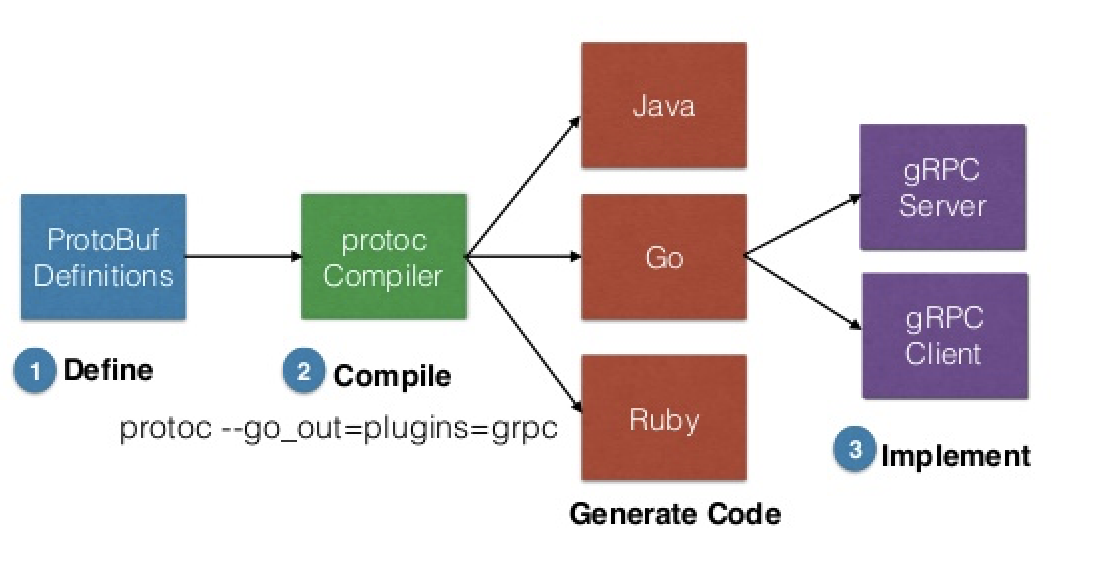
\includegraphics[width=9cm]{images/gRPCWorkflow}
\centering
\caption{gRPC \& Google Protocol Buffers Workflow}
\end{figure}


%----------------------------------------------------------------------------------------
%	Section 
%----------------------------------------------------------------------------------------

\section{Project Stages} % Numbered section

To implement a bulletin board service using gRPC and Google Protocol Buffers, we will break down this project into four stages:
\begin{itemize}  
\item Stage 1 – Generating Interface Classes using gRPC and Protocol Buffers
\item Stage 2 – Implementing the Bulletin Board Service
\item Stage 3 – Implementing the Bulletin Board Server
\item Stage 4 – Implementing the Bulletin Board Client 
\end{itemize}

%---------------------------------------------------------------------------------------


%----------------------------------------------------------------------------------------
%	Section 
%----------------------------------------------------------------------------------------

\section{Stage 1: Defining the Interface and generating the service classes} % Numbered section

Before we can implement anything, we need to define the interface for our service within a .proto file. We have to consider the messages our client and server will be passing back to each other. We will need a message to pass a post consisting of title and body. We will also need another message to represent a list of posts that the Server will send back to the client when the client asks for the list of posts. We will also need three RPCs: One for posting a post, one for getting a post, and one for listing the posts. To generate the service classes, follow the instructions to build your project in section 8.\\\\In general, for stage 1 you will need to:
\begin{itemize}
\item Define messages within the proto file
\item Define RPC services within the proto file
\item Build the project to generate gRPC classes
\end{itemize}
\begin{info}[Note:]
Make sure to read the entire project description, especially the section describing the client requirements as you will need to to get an idea of what RPCs should be defined in your Proto file.
\end{info}

%----------------------------------------------------------------------------------------

%----------------------------------------------------------------------------------------
%	Section 
%----------------------------------------------------------------------------------------

\section{Stage 2: Implementing the Bulletin Board Service} % Numbered section

The Google Protocol Compiler will generate the base classes your service will use. This will include classes implementation of the messages you defined and a gRPC class that implements the base of your service. In this case, if generated properly, there would be a grpc class that would have been generated. The filename would be prefixed with the name of the service you defined in the Proto file. Within this class there will be a static class with the suffix ImplBase. This class will have the RPC methods you have defined in the proto file. Your task is to extend this class with BulletinBoardService.java and override the RPC methods. \\\\In general, for stage 2 you will need to:
\begin{itemize}
\item Extend the generated *ImplBase Class with BulletinBoardService.java
\item Override all generated RPC methods
\item Implement a system to handle posts from clients
\end{itemize}

%----------------------------------------------------------------------------------------

%----------------------------------------------------------------------------------------
%	Section 
%----------------------------------------------------------------------------------------

\section{Stage 3: Implementing the Bulletin Board Server} % Numbered section

In order to use the service, you will have to create a server. The server will use the gRPC framework to instantiate a new Bulletin Board Service and bind it to a port.  Your task will be to implement this within BulletinBoardServer.java \\\\In general, for stage 3 you will need to:
\begin{itemize}
\item Figure out how to initialize and start a new RPC service
\end{itemize}

%----------------------------------------------------------------------------------------


%----------------------------------------------------------------------------------------
%	Section 
%----------------------------------------------------------------------------------------

\section{Stage 4: Implementing the Bulletin Board Client } % Numbered section

In order to interact with the Bulletin Board Service, you will need to create a client. Your task will be to implement this within BulletinBoardServer.java. The client will have make a stub object and connect to the service. The client will be able to invoke RPCs using the stub object.\\\\
The client should then take in the following commands:
\begin{itemize}
\item post <Title> <Body> - sends a post to our Bulletin Board Server with a title and body
\item get <Title> - gets the post and prints out the body
\item delete <Title> - deletes the post of the given title
\item list – lists all the post titles on the bulletin board \\
\end{itemize}
In general, for stage 4, you will need to:
\begin{itemize}
\item Figure out how to use the gRPC generated code to connect to the RPC Service
\item Figure out how to take in user input and invoke the proper RPCs
\item Format client output in a way that is readable and understandable\\
\end{itemize}

%----------------------------------------------------------------------------------------

\begin{figure}[h]
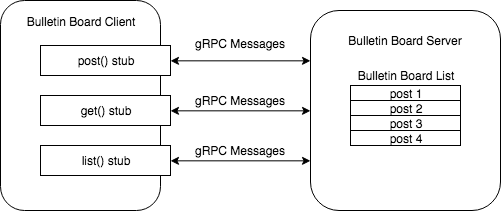
\includegraphics[width=10cm]{images/architecture}
\centering
\caption{Simple Bulletin Board Service Overview}
\end{figure}

%----------------------------------------------------------------------------------------
%	Section 
%----------------------------------------------------------------------------------------

\section{Getting Started} % Numbered section
The following sections describe how to get started on the project. 

\subsection{Requirements}
In order to complete this project you will need the following:
\begin{enumerate}
\item Java JDK
\item gRPC-BulletinBoard project template
\item Eclipse IDE (optional)
\end{enumerate}

\subsection{Downloading the Project Template}
If you do not already have the Project Template ZIP provided, you can download the project template two other ways:
\begin{itemize}
\item Download directly from Github:\\ https://github.com/DaveedDomingo/GRPC-Bulletin-Board-Project/archive/master.zip
\item Clone the project template using GIT:\\ git clone https://github.com/DaveedDomingo/GRPC-Bulletin-Board-Project.git
\end{itemize} 
The Project Template would be the folder labeled project-template

\subsection{Importing the Project into Eclipse}
To import the project into Eclipse, carry out the following steps:
\begin{enumerate}
\item In Eclipse Go to "File" > "Import"
\item Under the Maven folder, select “Existing Maven Projects”. Click Next
\item In “Root Directory”, browse to the gRPC-BulletinBoard-Project folder. If done correctly, there will be an entry under project window called /pom.xml
\item Ensure /pom.xml is selected. 
\item Click Finish.
\end{enumerate}
\begin{info}[Note:]
Eclipse may show errors within the project after importing into Eclipse, more specifically an error in the POM.xml file. To resolve this simply refresh the project by right clicking the project and seleting "refresh". New target folders should show up and the error should go away. 
\end{info}
\begin{info}[Eclipse is not mandatory:]
Although it is recommended, \textbf{it is not necessary to use the Eclipse IDE}. We are using Eclipse because it already comes prepackaged with Apache Maven. Maven is a tool that is used to help automate the building of a Java project. If you decide you do not want to use Eclipse you will still need Maven to build and compile the project. You can look up look up instructions on how to install the Maven tool on your particular operating system. We will mention how to use Maven in both Eclipse and Command Line in the following sections.
\end{info}

\subsection{Project Template Overview}

The following is the bare structure of the project template: \\

\dirtree{%
.1 project-template.
.2 src.
.3 main.
.4 java.
.5 com.
.6 bulletinboard.
.7 BulletinBoardService.java.
.7 BulletinBoardServer.java.
.7 BulletinBoardClient.java.
.4 proto.
.5 BulletinBoard.proto.
.2 pom.xml.
}

\begin{info}[Notice:]
If you imported the project into Ecllipse, additional folders may be present. This is due to Eclipse realizing that it is a Maven project, autogenerating extra folders that it may use.
\end{info}

\-\ \\Within the /src/main/proto directory there is one file:
\begin{itemize}
\item \textbf{\textit{BulletinBoard.proto}} - Here is where you will define the messages and services for the bulletin board\\  
\-\ \-\ \-\ \-\ \-\ \-\ \-\ \-\ \-\ \-\  \-\ \-\ \-\ \-\ \-\ \-\ \-\ \-\ \-\ \-\ \-\ \-\ \-\ \-\ \-\ \-\ \-\ \-\ \-\ \-\ \-\ \-\ \-\ \-\ \-\ \-\
service using google protocol buffer’s proto3 syntax
\end{itemize}

% File contents
\begin{file}[BulletinBoard.proto]
\begin{lstlisting}[]
1  syntax = "proto3";
2  package com.bulletinboard;
3  option java_multiple_files = true;
4
5  // Implement Proto File Here
\end{lstlisting}
\end{file}
Notice that this file comes with a few lines already present to help get you started. Line 2 has been added to ensure that generated gRPC source classes will already be automatically added to your build path, reliving the need to explicitly import them within your implementation classes. You will still however need to figure out which other gRPC packages to import to use the generated code. Line 3 has been added to ensure the Google Protocol Buffer compiler will generate code into multiple files. Without this, It will place all generated classes sources in a single file containing multiple classes. It's recommended not to change these lines\\

\-\ \\Within the /src/main/java/com/bulletinboard directory there are three files:
\begin{itemize}
\item \textbf{\textit{BulletinBoardService.java}} - This is where you will implement the RPC methods
\item \textbf{\textit{BulletinBoardServer.java}} - This is where you will implement the server application
\item \textbf{\textit{BulletinBoardClient.java}} - This is where you will implement the client application\\\\
\end{itemize}
You will notice at the root of the project there is a file called \textbf{\textit{pom.xml}}. This file is for Maven. Like mentioned in the previous section notice, Maven is a build tool used for Java projects and uses the pom.xml file to know how to build the Java project as well as know what dependencies need to downloaded before hand. \textbf{DO NOT EDIT THIS FILE}. The pom.xml file has been preconfigured to include the gRPC and google protocol buffer dependencies as well as preconfigured to generate gRPC code and Runnable JARs every time the project is compiled \textit{for your convenience}. 

%---------------------------------------------------------------------------------------



%----------------------------------------------------------------------------------------
%	Section 
%----------------------------------------------------------------------------------------

\section{Building the Project} % Numbered section
To build your project, you will need to use Maven and run "goals". Goals are procedures that carry out actions related to the project lifecycle. There are three Maven goals you will need will to familiarize yourself with in order to build and compile your project:
\begin{itemize}
\item install - this goal downloads any dependencies for your project
\item package - this goal compiles the project and packages artifacts.
\item clean - this goal cleans the project of any artifacts and code generated by the project
\end{itemize}

\subsection{Install}
The install goal downloads any dependencies and plugins you will need for your project. You will need to run this goal when you first import your project so the nessesary gRPC and Google Protocol Buffer libraries can be downloaded. If you don't do this, your IDE may give you errors or you may get errors when you try and build the project. 
\begin{itemize}
\item To do this in Eclipse:
	\begin{enumerate}
	\item In Eclipse, select the project folder within the Package Explorer window.
	\item Go to "Run" > "Run As" > "Maven Install"
	\end{enumerate}
\item To do this in Command Line:
	\begin{enumerate}
	\item Navigate to the root of the project directory.
	\item Run the following: "mvn install"
	\end{enumerate}
\end{itemize}

\subsection{Package}
The package goal will carry out the Maven build process: compiling project code, packaging artifacts, as well as carry out any additional tasks defined within the pom.xml file. You will need to run this goal for two reasons. The first is to generate gRPC Java code. Within the pom.xml there is a task that invokes the Google Protocol Buffer compiler to take the proto file you defined and generate Java classes. These classes are what you will use to implement your service. The second reason to run the package goal is to compile your server and client code so that you can run them.
\begin{itemize}
\item To do this in Eclipse:
	\begin{enumerate}
	\item In Eclipse, select the project folder within the Package Explorer window.
	\item Go to "Run" > "Run As" > "Maven build..."
	\item Within the Goals text box, type in "package"
	\item Click "Run" 
	\end{enumerate}
\item To do this in Command Line:
	\begin{enumerate}
	\item Navigate to the root of the project directory.
	\item Run the following: "mvn package"
	\end{enumerate}
\end{itemize}

\subsection{Clean}
The clean goal will clean the project directory of any generated project artifacts and source code. Project artifacts and generated code are usually placed within a folder named "target". You will need to run the clean goal before you build your project with the package goal to ensure any files from your old code is gone. You can run the package goal without running the clean goal as it will just overwrite the existing files, but there may be some files that were not overwritten still lying around.
\begin{itemize}
\item To do this in Eclipse:
	\begin{enumerate}
	\item In Eclipse, select the project folder within the Package Explorer window.
	\item Go to "Run" > "Run As" > "Maven clean"
	\end{enumerate}
\item To do this in Command Line:
	\begin{enumerate}
	\item Navigate to the root of the project directory.
	\item Run the following: "mvn clean"
	\end{enumerate}
\end{itemize}
\begin{info}[Note:]
Sometimes when running the previous goals in Eclipse, it may seem like nothing changed within the project structure. An example would be the target folder not showing up after you built your project. This is because Eclipse may have failed to update the window to reflect the new files. If this happens, try refreshing by right-clicking the project folder and selecting refresh. 
\end{info}

%----------------------------------------------------------------------------------------

%----------------------------------------------------------------------------------------
%	Section 
%----------------------------------------------------------------------------------------

\section{Running Your Project} % Numbered section
While you are implementing your service, you may want to test your server and client applications. \\
\begin{itemize}
\item To do this in Eclipse:
	\begin{enumerate}
	\item In Eclipse, right-click the BulletinBoardServer.java within the Package Explorer window.
	\item Run the server by selecting "Run As" > "Java Application"
	\item Repeat steps 1 and 2 but for the client class instead
	\end{enumerate}
\item To do this in Command Line:
	\begin{enumerate}
	\item Navigate to the root of the project directory.
	\item Navigate to the target folder where the runnable server and client jars should have been placed
	\item Run the server by running: java -jar BulletinBoardServer.jar
	\item Repeat step 3 but for the client jar instead. 
	\end{enumerate}
\end{itemize}

\subsection*{Sample execution}
The following is a sample of what the client output should look like:
% Command-line "screenshot"
\begin{commandline}
	\begin{verbatim}
		$ java -jar BulletinBoardClient.jar
		Client started. Connected to service at port 5501.
		Input a command: post  “Hello”  “This is a message to the world”
		Input a command: list
		Posts:
		     1. Hello
		Input a command: get “Hello”
		This is a message to the world
		Input a command: delete "Hello"
		Input a command: list
		There are no posts available.
		....
	\end{verbatim}
\end{commandline}
The following is a sample of what the server output should look like:
% Command-line "screenshot"
\begin{commandline}
	\begin{verbatim}
		$ java -jar BulletinBoardServer.jar
		Server started. Listening at port 5501.
		Posting post with title "Hello" and body "This is a message to the world"
		Deleting post "Hello"
		....
	\end{verbatim}
\end{commandline}
You will not have have to follow this format exactly. This is just an example. You can have the input and output be as formatted as much as you would like, given that it is simple and intuitive. What this means is that I should not need to ask questions or read any documentation to carry out the main functionalities the client should have.  

%----------------------------------------------------------------------------------------


%----------------------------------------------------------------------------------------
%	Section 
%----------------------------------------------------------------------------------------

\section{Submission } % Numbered section
To submit your project, have ONE of the group members submit two things:

\begin{enumerate}
\item \textbf{A zip file of your just the /src directory.} Compressing the whole project would be too much due to the downloaded libraries and generated artifacts and jars. It would come out to 200+ mb. The src directory with your implemented java classes as well as the proto file should be enough. I should be able to generate the source files with the Google Protocol Buffer compiler on the fly in order to build you project
\item \textbf{A pdf document consisting of the following 4 things:}
	\begin{itemize}
	\item List of group members
	\item A short paragraph or two describing what you accomplished including details on how to use the client if you deviated from the original design
	\item A short paragraph or two describing any issues you may have encountered and how you think you could have solved them. If you didn't have any simply state that you didn't have any issues.
	\item A few sentences to answer each the following two questions:
	\begin{enumerate}
		\item In this project, we implemented a simple RPC service but we didn't have to explicitly implement mechanisms to handle multiple clients. Instead we just used the mechanisms the gRPC framework provides. How does gRPC handle multiple clients?
		\item With the current implementation, if we add the requirement stating that each post title must be unique, we could end up with more than one post with the same title if two clients post at times close enough to each other. How can we modify our implementation to ensure this edge case won't occur?
	\end{enumerate}
	\end{itemize}
\end{enumerate}

%----------------------------------------------------------------------------------------

%----------------------------------------------------------------------------------------
%	Section 
%----------------------------------------------------------------------------------------

\section{Additional Hints} % Numbered section
\begin{info}[Tutorials are you friend:]
Follow gRPC tutorials to understand the syntax, design patterns, and development process when using generated gRPC code 
\end{info}
\begin{info}[Easy Method Overriding in Eclipse:]
After extending the base service class, you can easily override the methods in Eclipse by going to "Source" > "Override/Implement Methods...". This will show all superclasses and the inherited methods you can override. You can have eclipse automatically override any of the methods by selecting them and clicking 'Ok".
\end{info}
\begin{info}[Combining Maven Goals:]
You may find yourself running Maven goals frequently to build the project. You might find yourself running them so frequently it may just interfere with your precious development time. Luckily you can group goals together. For example, since it is good practice run the clean goal before the package goal, we should group them. In Eclipse this is done by running a Maven build like we are running the package goal, but instead of writing "package" in the Goals text box, we write "clean package". In Command Line, this is done by navigating the root of the project directory and running "mvn clean package". These will both run the clean goal first then the package goal. 
\end{info}
\begin{info}[When in doubt, Maven clean install package:]
Maven projects are complicated. If you're wondering why your code may not be running or compiling as intended, re-run the Maven goals to make sure the proper dependencies are installed and you're building in a fresh workspace. This way, if it still doesn't work, you can be sure it was because of your own doing.
\end{info}


%----------------------------------------------------------------------------------------

%----------------------------------------------------------------------------------------
%	Section 
%----------------------------------------------------------------------------------------

\section{Useful Links and Resources} % Numbered section
\begin{itemize}
\item \textbf{What is gRPC?} - https://grpc.io/docs/guides/
\item \textbf{gRPC Concepts} - https://grpc.io/docs/guides/concepts.html
\item \textbf{gRPC Java Quickstart} - https://grpc.io/docs/quickstart/java.html
\item \textbf{gRPC Java Tutorial} - https://grpc.io/docs/tutorials/basic/java.html
\item \textbf{gRPC Live Coding} - https://youtu.be/sdsabcI02LE?t=19m40s 
\item \textbf{Google Protocol Buffer Proto3 Syntax} - https://developers.google.com/protocol-buffers/docs/proto3
\end{itemize}

%----------------------------------------------------------------------------------------

%----------------------------------------------------------------------------------------
%	Section 
%----------------------------------------------------------------------------------------

\section{Additional Questions} % Numbered section
If you have any questions about the project or are having any issues, email me at David.Domingo@rutgers.edu

%----------------------------------------------------------------------------------------

%% File contents
%\begin{file}[hello.py]
%\begin{lstlisting}[language=Python]
%#! /usr/bin/python
%
%import sys
%sys.stdout.write("Hello World!\n")
%\end{lstlisting}
%\end{file}

\end{document}
